\documentclass[a4paper,14pt, unknownkeysallowed]{extreport}

\usepackage{cmap} % Улучшенный поиск русских слов в полученном pdf-файле
\usepackage[T2A]{fontenc} % Поддержка русских букв
\usepackage[utf8]{inputenc} % Кодировка utf8
\usepackage[english,russian]{babel} % Языки: русский, английский
\usepackage{enumitem}


\usepackage{threeparttable}

\usepackage[14pt]{extsizes}

\usepackage{caption}
\captionsetup{labelsep=endash}
\captionsetup[figure]{name={Рисунок}}

% \usepackage{ctable}
% \captionsetup[table]{justification=raggedleft,singlelinecheck=off}

\usepackage{amsmath}

\usepackage{geometry}
\geometry{left=30mm}
\geometry{right=10mm}
\geometry{top=20mm}
\geometry{bottom=20mm}

\usepackage{titlesec}
\titleformat{\section}
	{\normalsize\bfseries}
	{\thesection}
	{1em}{}
\titlespacing*{\chapter}{0pt}{-30pt}{8pt}
\titlespacing*{\section}{\parindent}{*4}{*4}
\titlespacing*{\subsection}{\parindent}{*4}{*4}

\usepackage{setspace}
\onehalfspacing % Полуторный интервал

\frenchspacing
\usepackage{indentfirst} % Красная строка

\usepackage{titlesec}
\titleformat{\chapter}{\LARGE\bfseries}{\thechapter}{20pt}{\LARGE\bfseries}
\titleformat{\section}{\Large\bfseries}{\thesection}{20pt}{\Large\bfseries}

\usepackage{multirow}
\usepackage{listings}
\usepackage{xcolor}

% Для листинга кода:
\lstset{%
	language=python,   					% выбор языка для подсветки	
	basicstyle=\small\sffamily,			% размер и начертание шрифта для подсветки кода
	numbers=left,						% где поставить нумерацию строк (слева\справа)
	numberstyle=\tiny,		   		% размер шрифта для номеров строк
	stepnumber=1,						% размер шага между двумя номерами строк
	numbersep=5pt,						% как далеко отстоят номера строк от подсвечиваемого кода
	frame=single,						% рисовать рамку вокруг кода
	tabsize=4,							% размер табуляции по умолчанию равен 4 пробелам
	captionpos=t,						% позиция заголовка вверху [t] или внизу [b]
	breaklines=true,					
	breakatwhitespace=true,				% переносить строки только если есть пробел
	backgroundcolor=\color{white},
	basicstyle=\footnotesize\ttfamily,
	keywordstyle=\color{blue},
	stringstyle=\color{red},
	commentstyle=\color{gray}
	showspaces=false,
    showstringspaces=false
}


\usepackage{pgfplots}
\usetikzlibrary{datavisualization}
\usetikzlibrary{datavisualization.formats.functions}


\lstset{
	literate=
	{а}{{\selectfont\char224}}1
	{б}{{\selectfont\char225}}1
	{в}{{\selectfont\char226}}1
	{г}{{\selectfont\char227}}1
	{д}{{\selectfont\char228}}1
	{е}{{\selectfont\char229}}1
	{ё}{{\"e}}1
	{ж}{{\selectfont\char230}}1
	{з}{{\selectfont\char231}}1
	{и}{{\selectfont\char232}}1
	{й}{{\selectfont\char233}}1
	{к}{{\selectfont\char234}}1
	{л}{{\selectfont\char235}}1
	{м}{{\selectfont\char236}}1
	{н}{{\selectfont\char237}}1
	{о}{{\selectfont\char238}}1
	{п}{{\selectfont\char239}}1
	{р}{{\selectfont\char240}}1
	{с}{{\selectfont\char241}}1
	{т}{{\selectfont\char242}}1
	{у}{{\selectfont\char243}}1
	{ф}{{\selectfont\char244}}1
	{х}{{\selectfont\char245}}1
	{ц}{{\selectfont\char246}}1
	{ч}{{\selectfont\char247}}1
	{ш}{{\selectfont\char248}}1
	{щ}{{\selectfont\char249}}1
	{ъ}{{\selectfont\char250}}1
	{ы}{{\selectfont\char251}}1
	{ь}{{\selectfont\char252}}1
	{э}{{\selectfont\char253}}1
	{ю}{{\selectfont\char254}}1
	{я}{{\selectfont\char255}}1
	{А}{{\selectfont\char192}}1
	{Б}{{\selectfont\char193}}1
	{В}{{\selectfont\char194}}1
	{Г}{{\selectfont\char195}}1
	{Д}{{\selectfont\char196}}1
	{Е}{{\selectfont\char197}}1
	{Ё}{{\"E}}1
	{Ж}{{\selectfont\char198}}1
	{З}{{\selectfont\char199}}1
	{И}{{\selectfont\char200}}1
	{Й}{{\selectfont\char201}}1
	{К}{{\selectfont\char202}}1
	{Л}{{\selectfont\char203}}1
	{М}{{\selectfont\char204}}1
	{Н}{{\selectfont\char205}}1
	{О}{{\selectfont\char206}}1
	{П}{{\selectfont\char207}}1
	{Р}{{\selectfont\char208}}1
	{С}{{\selectfont\char209}}1
	{Т}{{\selectfont\char210}}1
	{У}{{\selectfont\char211}}1
	{Ф}{{\selectfont\char212}}1
	{Х}{{\selectfont\char213}}1
	{Ц}{{\selectfont\char214}}1
	{Ч}{{\selectfont\char215}}1
	{Ш}{{\selectfont\char216}}1
	{Щ}{{\selectfont\char217}}1
	{Ъ}{{\selectfont\char218}}1
	{Ы}{{\selectfont\char219}}1
	{Ь}{{\selectfont\char220}}1
	{Э}{{\selectfont\char221}}1
	{Ю}{{\selectfont\char222}}1
	{Я}{{\selectfont\char223}}1
}

\usepackage{graphicx}
\newcommand{\img}[3] {
	\begin{figure}[h!]
		\center{\includegraphics[height=#1]{img/#2}}
		\caption{#3}
		\label{img:#2}
	\end{figure}
}


\usepackage[justification=centering]{caption} % Настройка подписей float объектов

\usepackage[unicode,pdftex]{hyperref} % Ссылки в pdf
\hypersetup{hidelinks}

\usepackage{csvsimple}

\newcommand{\code}[1]{\texttt{#1}}

\usepackage{longtable}

\usepackage{array}
\usepackage{booktabs}
\usepackage{floatrow}

\floatsetup[longtable]{LTcapwidth=table}



\begin{document}


\begin{titlepage}
	\newgeometry{pdftex, left=2cm, right=2cm, top=2.5cm, bottom=2.5cm}
	\fontsize{12pt}{12pt}\selectfont
	\noindent \begin{minipage}{0.15\textwidth}
		
\includegraphics[width=\linewidth]{img/b_logo.jpg}
	\end{minipage}
	\noindent\begin{minipage}{0.9\textwidth}\centering
		\textbf{Министерство науки и высшего образования Российской Федерации}\\
		\textbf{Федеральное государственное бюджетное образовательное учреждение высшего образования}\\
		\textbf{«Московский государственный технический университет имени Н. Э.~Баумана}\\
		\textbf{(национальный исследовательский университет)»}\\
		\textbf{(МГТУ им. Н. Э.~Баумана)}
	\end{minipage}
	
	\noindent\rule{18cm}{3pt}
	\newline\newline
	\noindent ФАКУЛЬТЕТ $\underline{\text{«Информатика и системы управления»~~~~~~~~~~~~~~~~~~~~~~~~~~~~~~~~~~~~~~~~~~~~~~~~~~~~~~~}}$ \newline\newline
	\noindent КАФЕДРА $\underline{\text{«Программное обеспечение ЭВМ и информационные технологии»~~~~~~~~~~~~~~~~~~~~~~~}}$\newline\newline\newline\newline\newline\newline\newline
	
	
	\begin{center}
		\noindent\begin{minipage}{1.3\textwidth}\centering
		\Large\textbf{   ~~~ Лабораторная работа №7}\newline
		\textbf{по дисциплине "Анализ Алгоритмов"}\newline\newline\newline
		\end{minipage}
	\end{center}
	
	\noindent\textbf{Тема} 			$\underline{\text{Поиск в словаре}}$\newline\newline
	\noindent\textbf{Студент} 		$\underline{\text{Ковалец К. Э.}}$\newline\newline
	\noindent\textbf{Группа} 		$\underline{\text{ИУ7-53Б}}$\newline\newline
	\noindent\textbf{Преподаватель} $\underline{\text{Волкова Л. Л.}}$\newline
	
	\begin{center}
		\vfill
		Москва~---~\the\year
		~г.
	\end{center}
	\restoregeometry
\end{titlepage}



\renewcommand{\contentsname}{Содержание} 
\tableofcontents
\setcounter{page}{2}





\chapter*{Введение}
\addcontentsline{toc}{chapter}{Введение}

Словарь -- абстрактный тип данных, позволяющий хранить пары вида <<ключ -- значение>> и поддерживающий операции добавления пары, а также поиска и удаления пары по ключу.
В паре ($k$, $v$) значение $v$ называется значением, ассоциированным с ключом $k$. Поиск -- основная задача при использовании словаря. Данная задача решается различными способами, которые отличаются временем выполнения.

Целью данной лабораторной работы является изучение алгоритмов поиска в словаре – полным перебором, бинарным поиском и поиском сегментами. 

Для достижения поставленной цели необходимо выполнить следующие задачи:

\begin{itemize}
	\item исследовать понятие словаря;
	\item изучить алгоритмы поиска в словаре (перебором, бинарным поиском, сегментами);
	\item привести схемы используемых алгоритмов;
	\item описать используемые структуры данных;
	\item описать структуру разрабатываемого ПО;
	\item определить средства программной реализации;
	\item реализовать разработанные алгоритмы;
	\item провести функциональное тестирование;
	\item провести сравнительный анализ времени работы алгоритмов;
	\item описать и обосновать полученные результаты в отчете о выполненной лабораторной работе.
\end{itemize}





\chapter{Аналитическая часть}

В данном разделе будет представлено описание понятия словаря и описаны алгоритмы поиска в нём (полным перебором, бинарным поиском, поиском сегментами).

\section{Словарь}

Словарь [1] -- абстрактный тип данных, позволяющий хранить пары вида <<ключ -- значение>> и поддерживающий операции добавления пары, а также поиска и удаления пары по ключу.
В паре ($k$, $v$) значение $v$ называется значением, ассоциированным с ключом $k$.

Поиск -- основная задача при использовании словаря. Данная задача решается различными способами, которые отличаются временем выполнения.

В данной лабораторной работе использовался словарь со  следующими параметрами:

\begin{itemize}
	\item ключ - фамилия клиента;
	\item значение - информация о клиенте:
	\begin{itemize}
		\item имя;
		\item почта;
		\item телефон.
	\end{itemize}
\end{itemize}

\section{Алгоритм поиска полным перебором}

Поиск полным перебором [2] -- метод решения, при котором поочередно перебираются все ключи словаря, пока не будет найден нужный.

Сложность такого алгоритма зависит от количества всех возможных решений, а время решения может стремиться к экспоненциальному времени работы.
Чем дальше искомый ключ от начала словаря, тем выше трудоемкость алгоритма. Пусть на старте алгоритм затрагивает $k_0$ операций, а при сравнении $k_1$ операций, тогда:
\begin{itemize}
	\item в лучшем случае элемент будет найден на первом сравнении за $k_0 + k_1$ операций;
	\item в худшем случае элемент будет найден на последнем сравнении за $k_0 +  N \cdot k_1$ операций, где $N$ -- размер словаря;
	\item элемент будет найден на \textit{i-ом} сравнении за $k_0 + i \cdot k_1$ операций;
\end{itemize}

Тогда средняя трудоемкость может быть рассчитана по следующей формуле:

\begin{equation}
	f = k_0 + k_1 \cdot \left(1 + \frac{N}{2} - \frac{1}{N + 1}\right)
\end{equation}

\section{Алгоритм бинарного поиска}


Бинарный поиск [3] -- поиск в заранее отсортированном словаре, который заключается в сравнении со средним элементом, и, если ключ меньше, то продолжать поиск в левой части тем же методом, иначе -- в правой части.

Пусть на старте алгоритм затрагивает $k_0$ операций, тогда:
\begin{itemize}
	\item в лучшем случае элемент будет найден на первом сравнении с средним элементом с трудоемкостью $k_0 + \log_2 1$;
	\item в худшем случае элемент будет найден на последнем сравнении с трудоёмкостью $b +  \log_2 N$, где $N$ -- размер словаря;
	\item элемент будет найден на \textit{i-ом} сравнении с трудоемкостью $b + \log_2 i$;
\end{itemize}

В случае большого объема данных и обратного порядка сортировки может произойти так, что алгоритм полного перебора будет эффективнее по времени, чем алгоритм двоичного поиска.

\clearpage

\section{Алгоритм поиска сегментами}

Поиск с помощью сегментов [4] -- словарь разбивается на части, в каждую из которых попадают все элементы с некоторым общим признаком (для букв это может быть первая буква, для чисел -- остаток от деления).

Обращение к сегменту равно сумме вероятностей обращения к его ключам. Пусть $P_i$ -- вероятность обращения к $i$-ому сегменту, а $p_j$ -- вероятность обращения к $j$-ому элементу $i$-ого сегмента. Тогда вероятность выбрать нужный сегмент высчитывается так 

\begin{equation}
	P_i = \sum_j p_j
\end{equation}

Затем ключи в каждом сегменте сортируются, чтобы внутри каждого сегмента можно было произвести бинарный поиск с сложностью $O(\log_2 k)$, где $k$ -- количество ключей в сегменте.

То есть, сначала выбирается нужный сегмент, а затем в нём с помощью бинарного поиска ищется нужный ключ.

В лучшем случае первым сегментом будет выбран тот, серединный элемент которого окажется нужным.

В худшем случае последним сегментом будет выбран тот, который будет содержать нужный элемент, при этом сложность поиска ключа в данном сегменте -- $\log_2 N$, где $N$ - число элементов в сегменте.

Тогда средняя трудоемкость поиска $i$-го элемента может быть рассчитана по следующей формуле:
\begin{equation}
	\sum_{i \in \Omega}{\left(f_{\text{выбор сегмента i-ого элемента}} + f_{\text{бинарный поиск i-ого элемента}}\right)} \cdot p_i
\end{equation}

\clearpage

\section{Вывод}

В этом разделе были описаны понятие словаря и алгоритмы поиска в нём (полным перебором, бинарным поиском, поиском сегментами).

На вход программе будет поступать словарь (в нужной форме для каждого конкретного алгоритма), а также ключ, по которому будет происходить поиск в словаре. При попытке задать некорректные данные, будет выдано сообщение об ошибке. Если клинт с заданным ключом не будет найден, то выведется соответствующее сообщение. Реализуемое ПО будет давать возможность выбрать алгоритм поиска в словаре (полным перебором, бинарным поиском, поиском сегментами) и вывести для него результат вычисления, а также возможность произвести сравнение алгоритмов по затраченному времени и кол-ву используемых сравнений.





\chapter{Конструкторская часть}

В данном разделе будут приведены схемы алгоритмов поиска в словаре (полным перебором, бинарным поиском, поиском сегментами), приведено описание используемых типов данных, классов эквивалентности, а также описана структура ПО.

\section{Схемы алгоритмов}

На рис. \ref{fig:full_search} - \ref{fig:segment_search} приведены схемы алгоритмов поиска в словаре (полным перебором, бинарным поиском, поиском сегментами).

\begin{figure}[h]
	\centering
	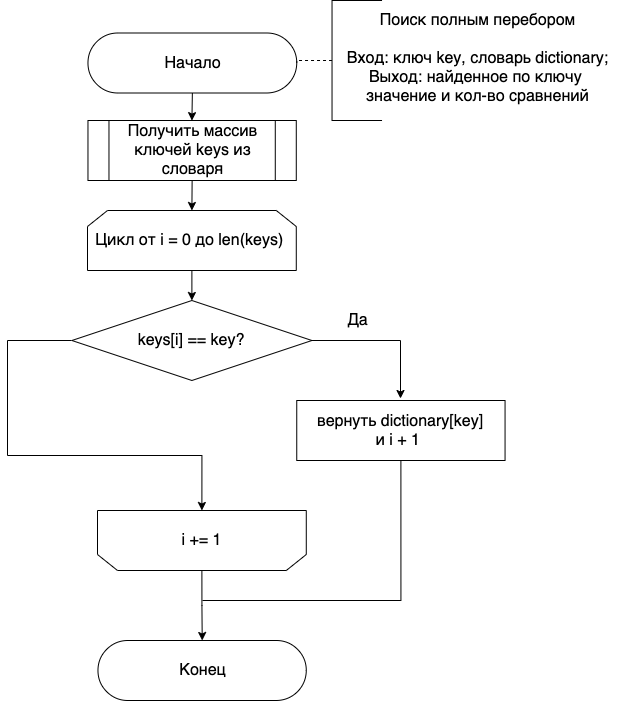
\includegraphics[scale=0.6]{img/full_search_scheme.png}
	\caption{Схема алгоритма поиска полным перебором}
	\label{fig:full_search}
\end{figure}

\clearpage

\begin{figure}[h]
	\centering
	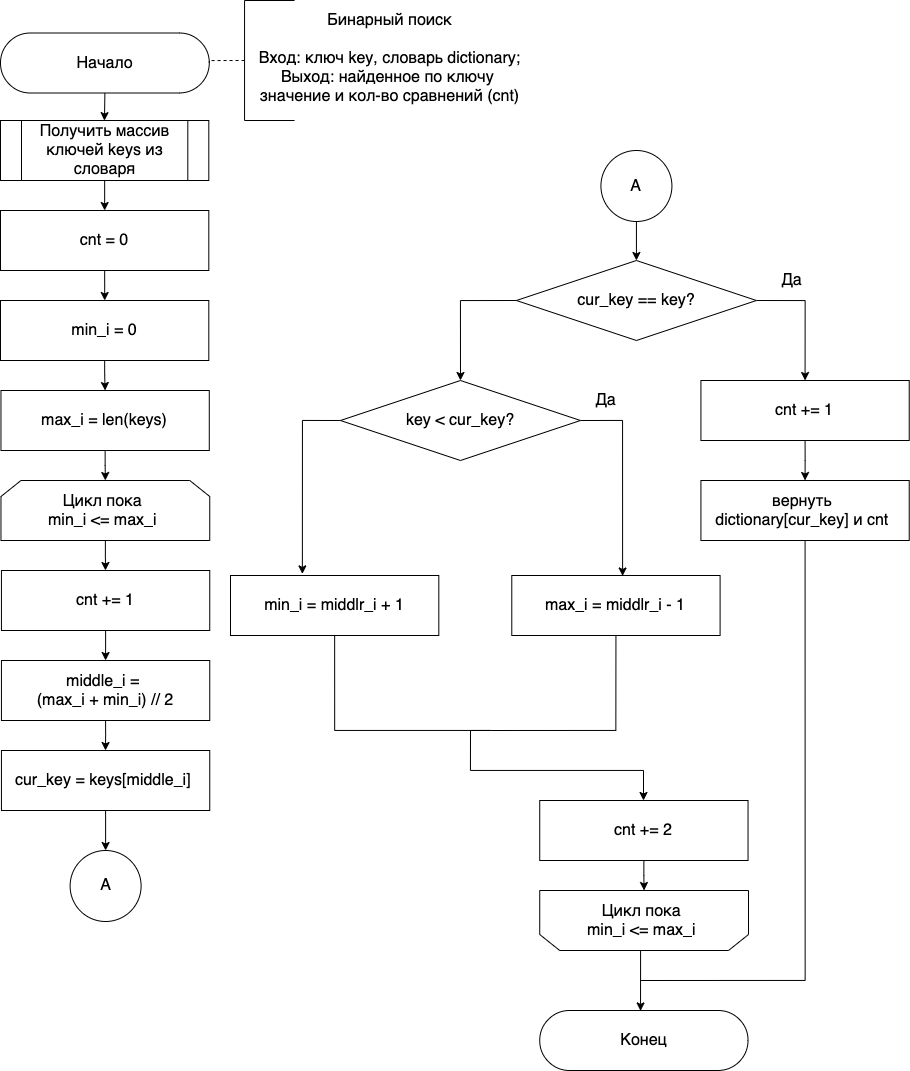
\includegraphics[scale=0.54]{img/binary_search_scheme.png}
	\caption{Схема алгоритма бинарного поиска}
	\label{fig:binary_search}
\end{figure}

\clearpage

\begin{figure}[h]
	\centering
	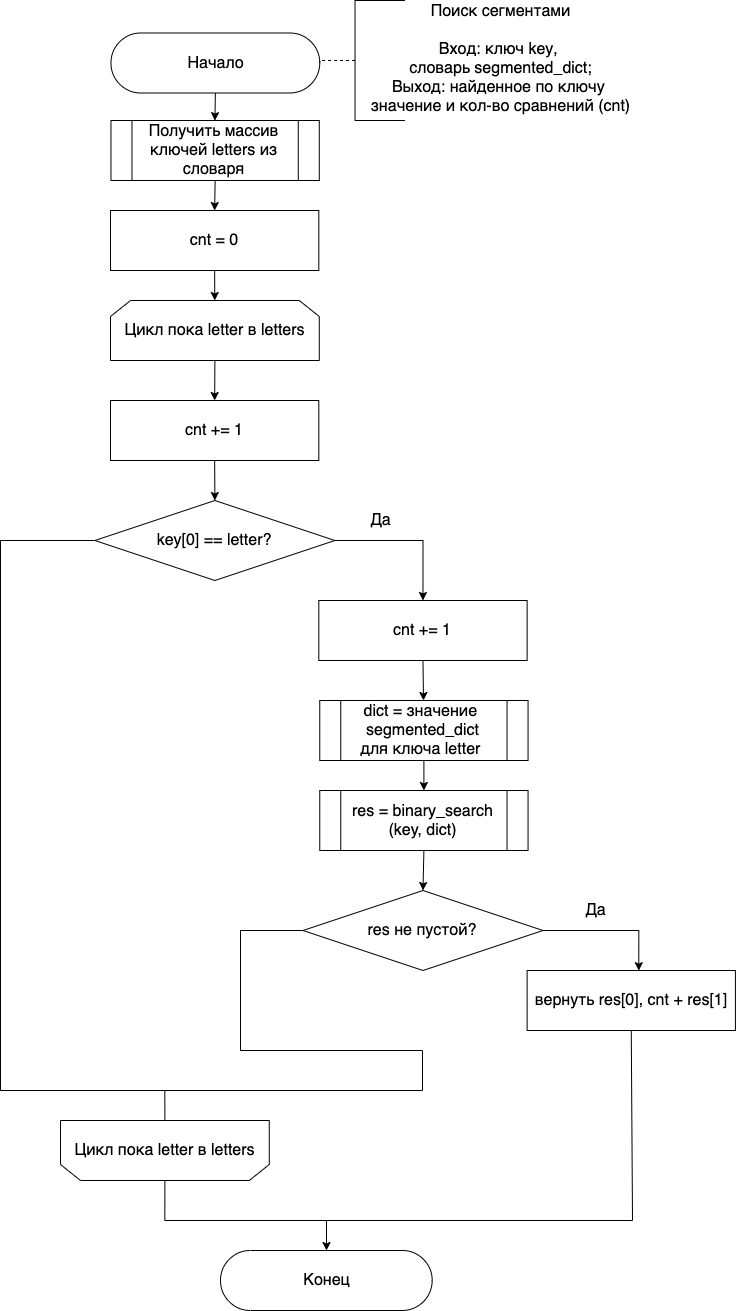
\includegraphics[scale=0.53]{img/segment_search_scheme.png}
	\caption{Схема алгоритма поиска сегментами}
	\label{fig:segment_search}
\end{figure}

\clearpage


\section{Классы эквивалентности}

Выделенные классы эквивалентности для тестирования:

\begin{itemize}
	\item номер команды < 0 или > 5;
	\item номер команды не является целым числом;
	\item в словаре нет введённого ключа;
	\item в словаре есть введённый ключ.
\end{itemize}

\section{Описание используемых типов данных}

При реализации алгоритмов будут использованы следующие структуры данных:

\begin{itemize}
	\item словарь - встроенный тип данных $dict$ для словаря в $Python$;
	\item ключ в словаре - строка типа $str$;
	\item значение в словаре - строка типа $str$;
	\item название файла - строка типа $str$.
\end{itemize}


\section{Структура ПО}

Реализуемое ПО будет давать возможность выбрать алгоритм поиска в словаре (полным перебором, бинарным поиском, поиском сегментами) и вывести для него результат вычисления, а также возможность произвести сравнение алгоритмов по затраченному времени и кол-ву используемых сравнений. Для взаимодействия с пользователем будет разработано меню. В данном ПО будет реализован метод структурного программирования. \newline

Для данного ПО будут разработаны следующие функции:

\begin{itemize}
	\item функция для генерации файла с данными о клиентах, входные данные - имя создаваемого файла;
    \item функция для создание словаря, использующая информацию из файла, входные данные - имя файла, выходные - заполненный словарь;
    \item функции для реализации алгоритмов поиска значений в словаре по ключу (полным перебором, бинарным поиском, поиском сегментами), входные данные - ключ, словарь, выходные - значение в словере по заданному ключу, кол-во сравнений, использованных в данном алгоритме;
    \item функция для вывода найденного значения словаря по ключу, а также кол-ва используемых алгоритмом сравнений, входные данные - ключ, значение словаря, кол-во сравнений;
    \item функция создания сегментного словаря для использования алгоритма поиска сегментами, входные данные - словарь, выходные - сегментный словарь;
    \item функция сортировки элементов словаря по ключу, входные данные - словарь, выходные - отсортированный словарь;
    \item функция для построения гистограмм кол-ва сравнений, используемых каждым из алгоритмов;
    \item функция для построения графика зависимости времени работы алгоритмов от индекса ключа.
\end{itemize}

\section{Вывод}

В данном разделе на основе теоретических данных были построены схемы требуемых алгоритмов поиска в словаре (полным перебором, бинарным поиском, поиском сегментами), выбраны используемые типы данных, выделены классы эквивалентности для тестирования, а также была описана структура ПО.

\clearpage





\chapter{Технологическая часть}

В данном разделе будут приведены средства реализации, cведения о модулях программы, листинги кода, а также функциональные тесты.


\section{Средства реализации}

В данной работе для реализации был выбран язык программирования $Python$ [5]. Выбор обсуловлен наличием опыта работы с ним. Время работы было замерено с помощью функции \textit{process\_time} из библиотеки $time$ [6].

\section{Сведения о модулях программы}

ПО будет состоять из следующих модулей:

\begin{itemize}
	\item $main.py$ -- файл, содержащий функцию $main$;
	\item $generate.py$ -- файл, содержащий функции для генирации файлов с данными о клиентах;
    \item $alg\_search.py$ -- файл, в котором содержатся функции реализаций алгоритмов поиска значений в словаре по ключу;
    \item $dictionary.py$ -- файл, в котором содержатся функции для работы со словарём;
    \item $compare.py$ -- файл, в котором содержатся функции для сравнения кол-ва сравнений внутри алгоритмов, замера времени работы алгоритмов и построения графика зависимоти времени выполнения от индекса ключа в словаре;
    \item $read.py$ -- файл, в котором содержатся функции ввода данных;
    \item $color.py$ -- файл, который содержит переменные типа $string$ для цветного вывода результата работы программы в консоль.
\end{itemize}

\section{Листинги кода}

В листингах \ref{lst:full_search} - \ref{lst:segment_search} представлены функции реализации алгоритмов поиска в словаре (полным перебором, бинарным поиском, поиском сегментами). В листинге \ref{lst:segment_dict}
представлена функция создания словаря для использования поиска по нему сегментами.

\begin{center} 
\captionsetup{justification=raggedright,singlelinecheck=off}
\begin{lstlisting}[label=lst:full_search,caption=Алгоритм поиска полным перебором]
def full_search(key, dictionary):
    keys = list(dictionary.keys())

    for i in range(len(keys)):
        if keys[i] == key:
            return dictionary[key], i + 1
\end{lstlisting}
\end{center}	


\begin{center}
\captionsetup{justification=raggedright,singlelinecheck=off}
\begin{lstlisting}[label=lst:binary_search,caption=Алгоритм бинарного поиска]
def binary_search(key, dictionary):
    keys = list(dictionary.keys())

    cnt = 0
    min_i = 0
    max_i = len(keys)

    while min_i <= max_i:
        cnt += 1

        middle_i = (max_i + min_i) // 2
        cur_key = keys[middle_i]

        if cur_key == key:
            cnt += 1

            return dictionary[cur_key], cnt

        elif key < cur_key:
            max_i = middle_i - 1
        else:
            min_i = middle_i + 1

        cnt += 2
\end{lstlisting}
\end{center}

\clearpage

\begin{center}
\captionsetup{justification=raggedright,singlelinecheck=off}
\begin{lstlisting}[label=lst:segment_search,caption=Алгоритм поиска сегментами]
def segment_search(key, segmented_dict):
    letters = list(segmented_dict.keys())

    cnt = 0

    for letter in letters:
        cnt += 1  

        if key[0] == letter:
            cnt += 1  
            res = binary_search(key, segmented_dict.get(letter))

            if res is not None:
                return res[0], cnt + res[1]
\end{lstlisting}
\end{center}	

\begin{center}
\captionsetup{justification=raggedright,singlelinecheck=off}
\begin{lstlisting}[label=lst:segment_dict,caption=Функция создания словаря для использования поиска по нему сегментами]
def segment_dict(dictionary):
    tmp_dict = {i: 0 for i in "ЙЦУКЕНГШЩЗХФЫВАПРОЛДЖЭЁЯЧСМИТБЮ"}

    for key in dictionary:
        tmp_dict[key[0]] += 1

    tmp_dict = sort_dict_by_data(tmp_dict)

    segmented_dict = tmp_dict

    for key in segmented_dict:
        segmented_dict[key] = dict()

    for key in dictionary:
        segmented_dict[key[0]].update({key: dictionary[key]})

    return segmented_dict
\end{lstlisting}
\end{center}

\clearpage

\section{Функциональные тесты}

В таблице \ref{tbl:functional_test} приведены функциональные тесты для алгоритмов поиска в словаре (полным перебором, бинарным поиском, поиском сегментами). Все тесты пройдены успешно.

\begin{center}
\captionsetup{justification=raggedright,singlelinecheck=off}
\begin{longtable}[c]{|c|c|c|}
\caption{Функциональные тесты\label{tbl:functional_test}}
	\\ \hline
	Входные данные & Алгоритм & Результат 
	\\ \hline
	команда 10 &  & Сообщение об ошибке
	\\ \hline
	команда k &  & Сообщение об ошибке
	\\ \hline
	"Морозова" & Полный перебор & Такого клиента нет
	\\ \hline
	"Морозова" & Бинарный поиск & Такого клиента нет
	\\ \hline
	"Морозова" & Поиск сегментами & Такого клиента нет
	\\ \hline
	"Петров" (случайный ключ) & Полный перебор & Информация о клиенте
	\\ \hline
	"Петров" (случайный ключ) & Бинарный поиск & Информация о клиенте
	\\ \hline
	"Петров" (случайный ключ) & Поиск сегментами & Информация о клиенте
	\\ \hline
	"Аалферов" (первый ключ) & Полный перебор & Информация о клиенте
	\\ \hline
	"Аалферов" (первый ключ) & Бинарный поиск & Информация о клиенте
	\\ \hline
	"Аалферов" (первый ключ) & Поиск сегментами & Информация о клиенте
	\\ \hline
	"Яяпмей" (последний ключ) & Полный перебор & Информация о клиенте
	\\ \hline
	"Яяпмей" (последний ключ) & Бинарный поиск & Информация о клиенте
	\\ \hline
	"Яяпмей" (последний ключ) & Поиск сегментами & Информация о клиенте
	\\ \hline
\end{longtable}
\end{center}

\section{Вывод}

В данном разделе были разработаны алгоритмы поиска в словаре (полным перебором, бинарным поиском, поиском сегментами), проведено тестирование, описаны средства реализации и cведения о модулях программы.





\chapter{Исследовательская часть}

\section{Технические характеристики}

Технические характеристики устройства, на котором выполнялось тестирование представлены далее.

\begin{itemize}
    \item Операционная система: macOS 11.5.2. [7]
    \item Память: 8 GiB.
    \item Процессор: 2,3 GHz 4-ядерный процессор Intel Core i5. [8]
\end{itemize}

При тестировании ноутбук был включен в сеть электропитания. Во время тестирования ноутбук был нагружен только встроенными приложениями окружения, а также системой тестирования.

\section{Демонстрация работы программы}

\img{80mm}{example}{Пример работы программы}

\clearpage

\section{Время выполнения алгоритмов}

Результаты замеров времени работы алгоритмов поиска в словаре (полным перебором, бинарным поиском, поиском сегментами) представлены на рисунках 4.2 - 4.3. Замеры времени проводились в секундах и усреднялись для каждого набора одинаковых экспериментов.

\img{40mm}{time}{Замеры времени работы алгоритмов поиска в словаре}

\img{125mm}{graph_time}{Зависимость времени работы алгоритмов поиска от индекса ключа}

\clearpage

\section{Кол-во сравнений при работе алгоритмов}

Для каждого алгоритма был проведён анализ по количеству сравнений для нахождения каждого ключа в словаре. Были составлены по две гистограммы для всех алгоритмов поиска (ключи расположены в том же порядке, как и в словаре, и когда ключи отсортировнны в порядке убывания).


\begin{figure}[h]
	\centering
	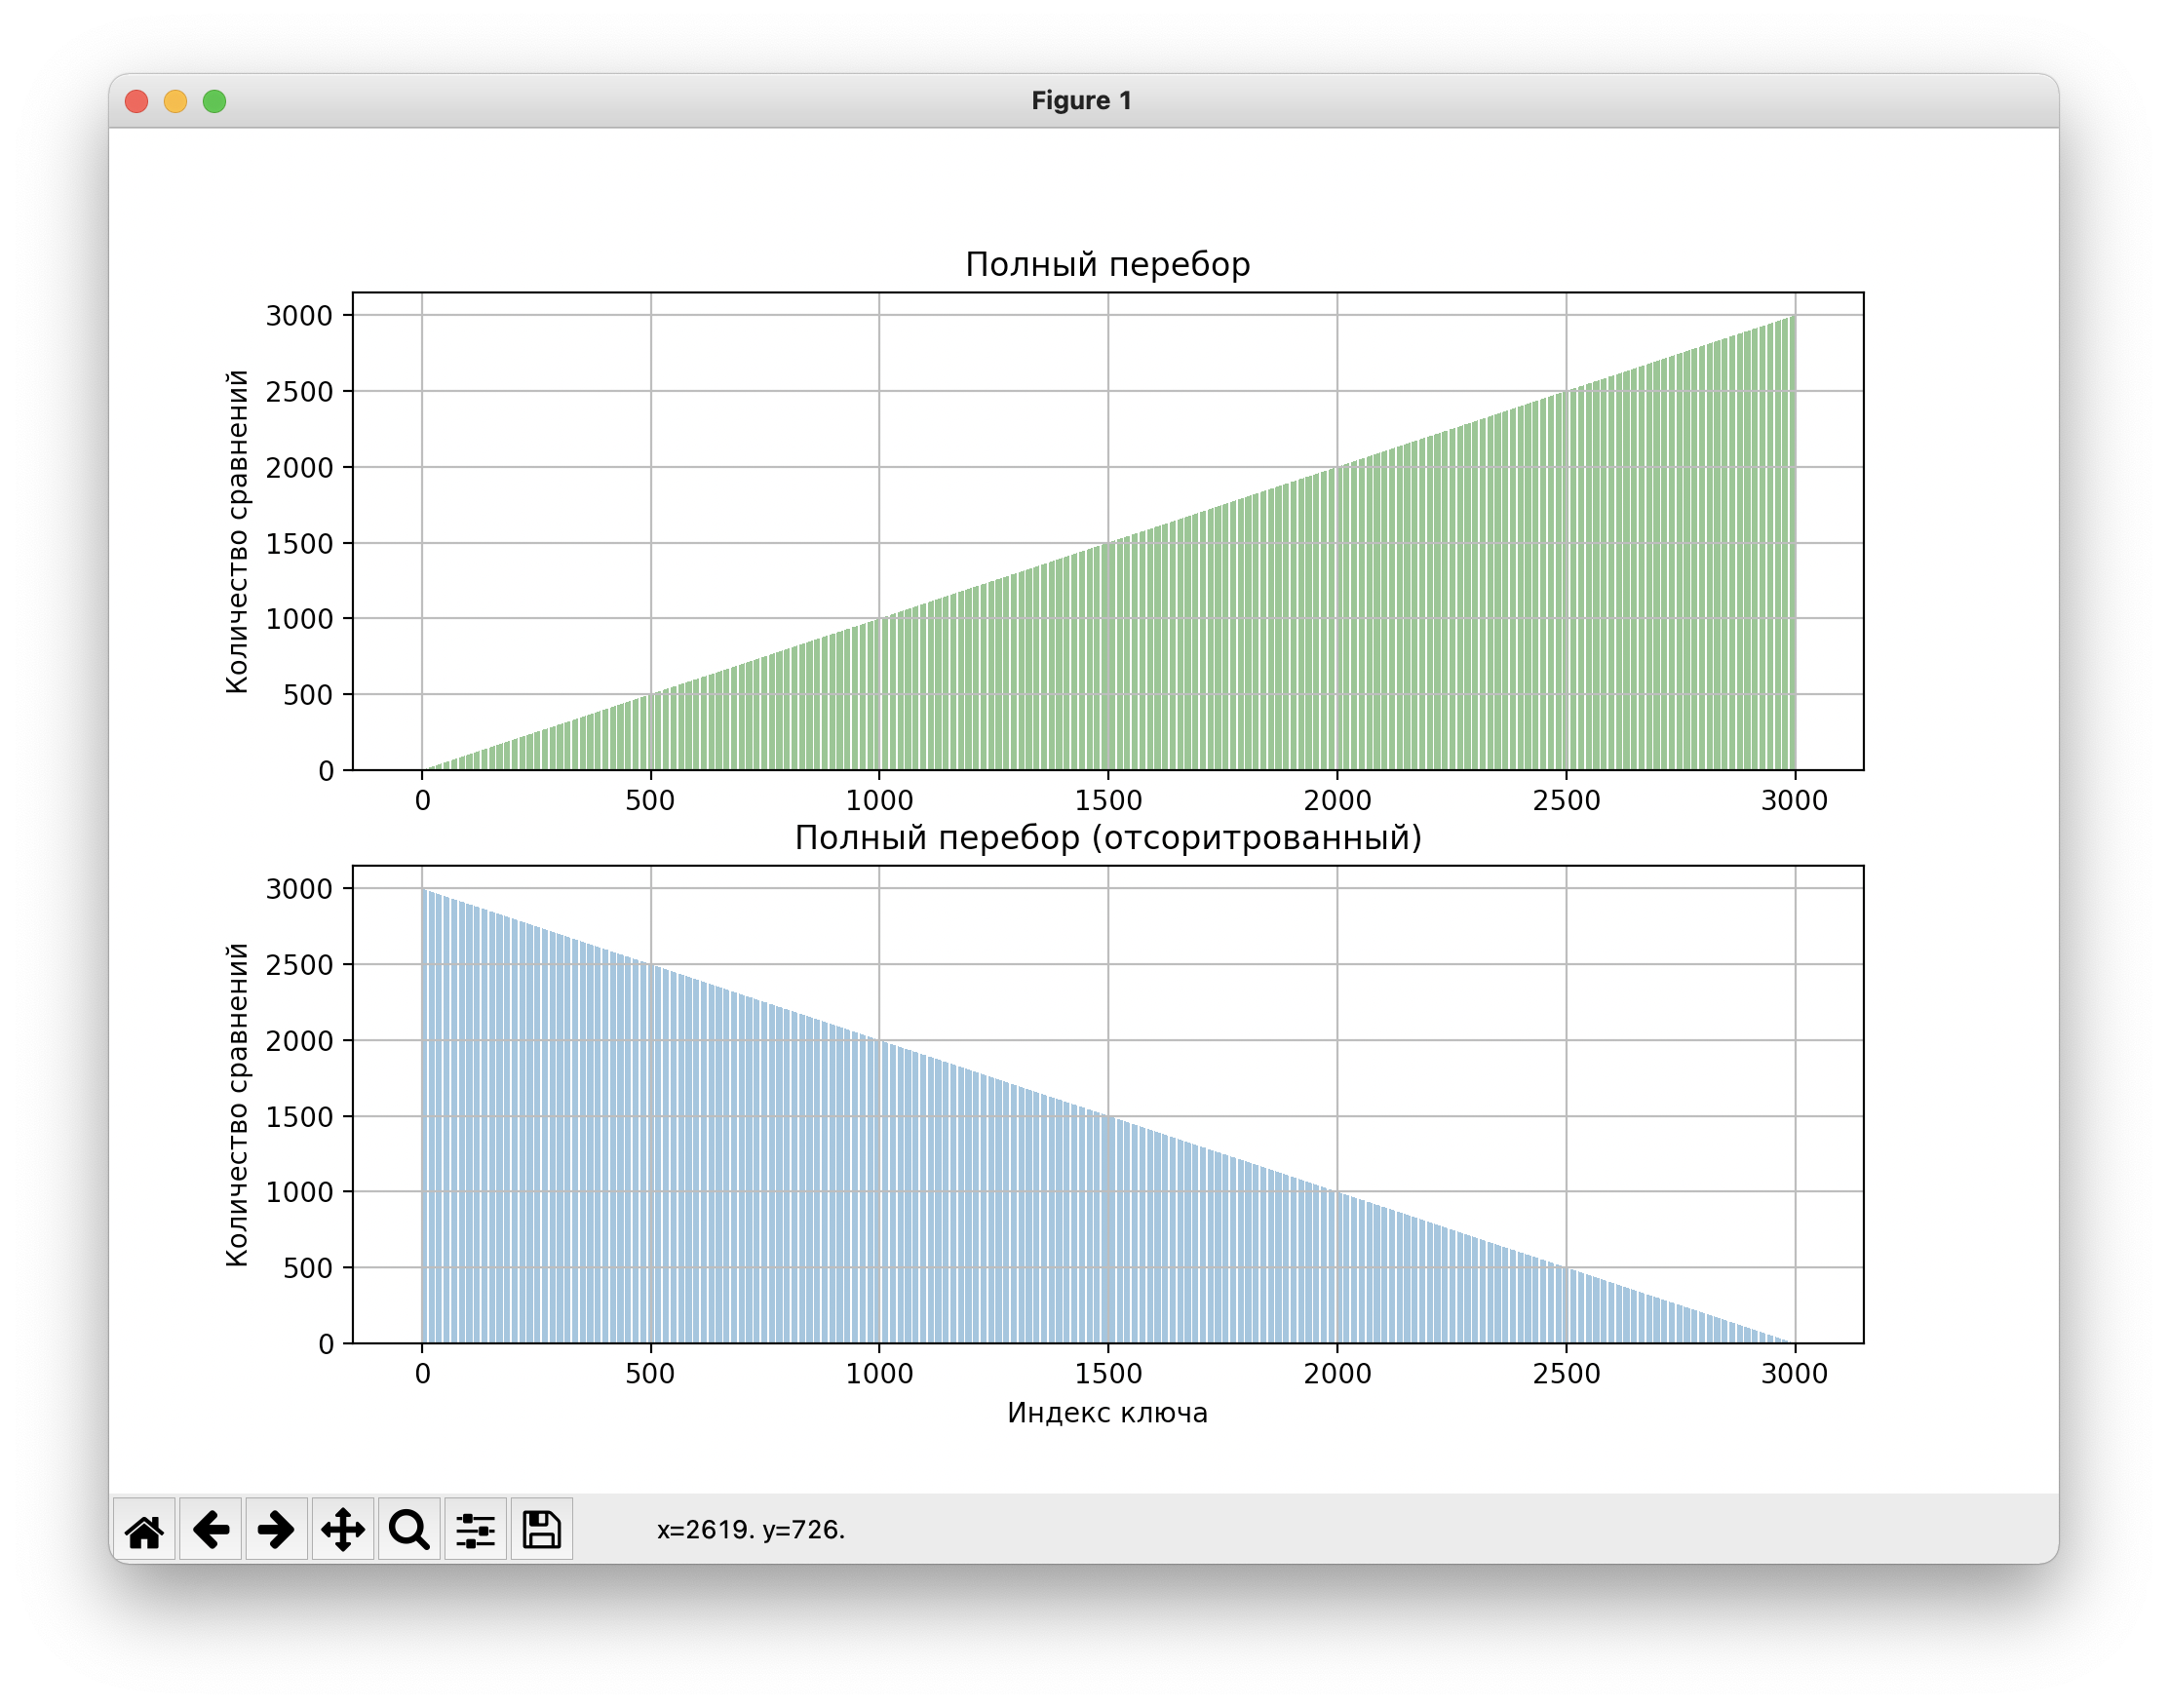
\includegraphics[scale=0.45]{img/graph_full_search.png}
	\caption{Кол-во сравнений при поиске ключа в словаре (полным перебором)}
	\label{fig:graph_full_search}
\end{figure}

\clearpage

\begin{figure}[h]
	\centering
	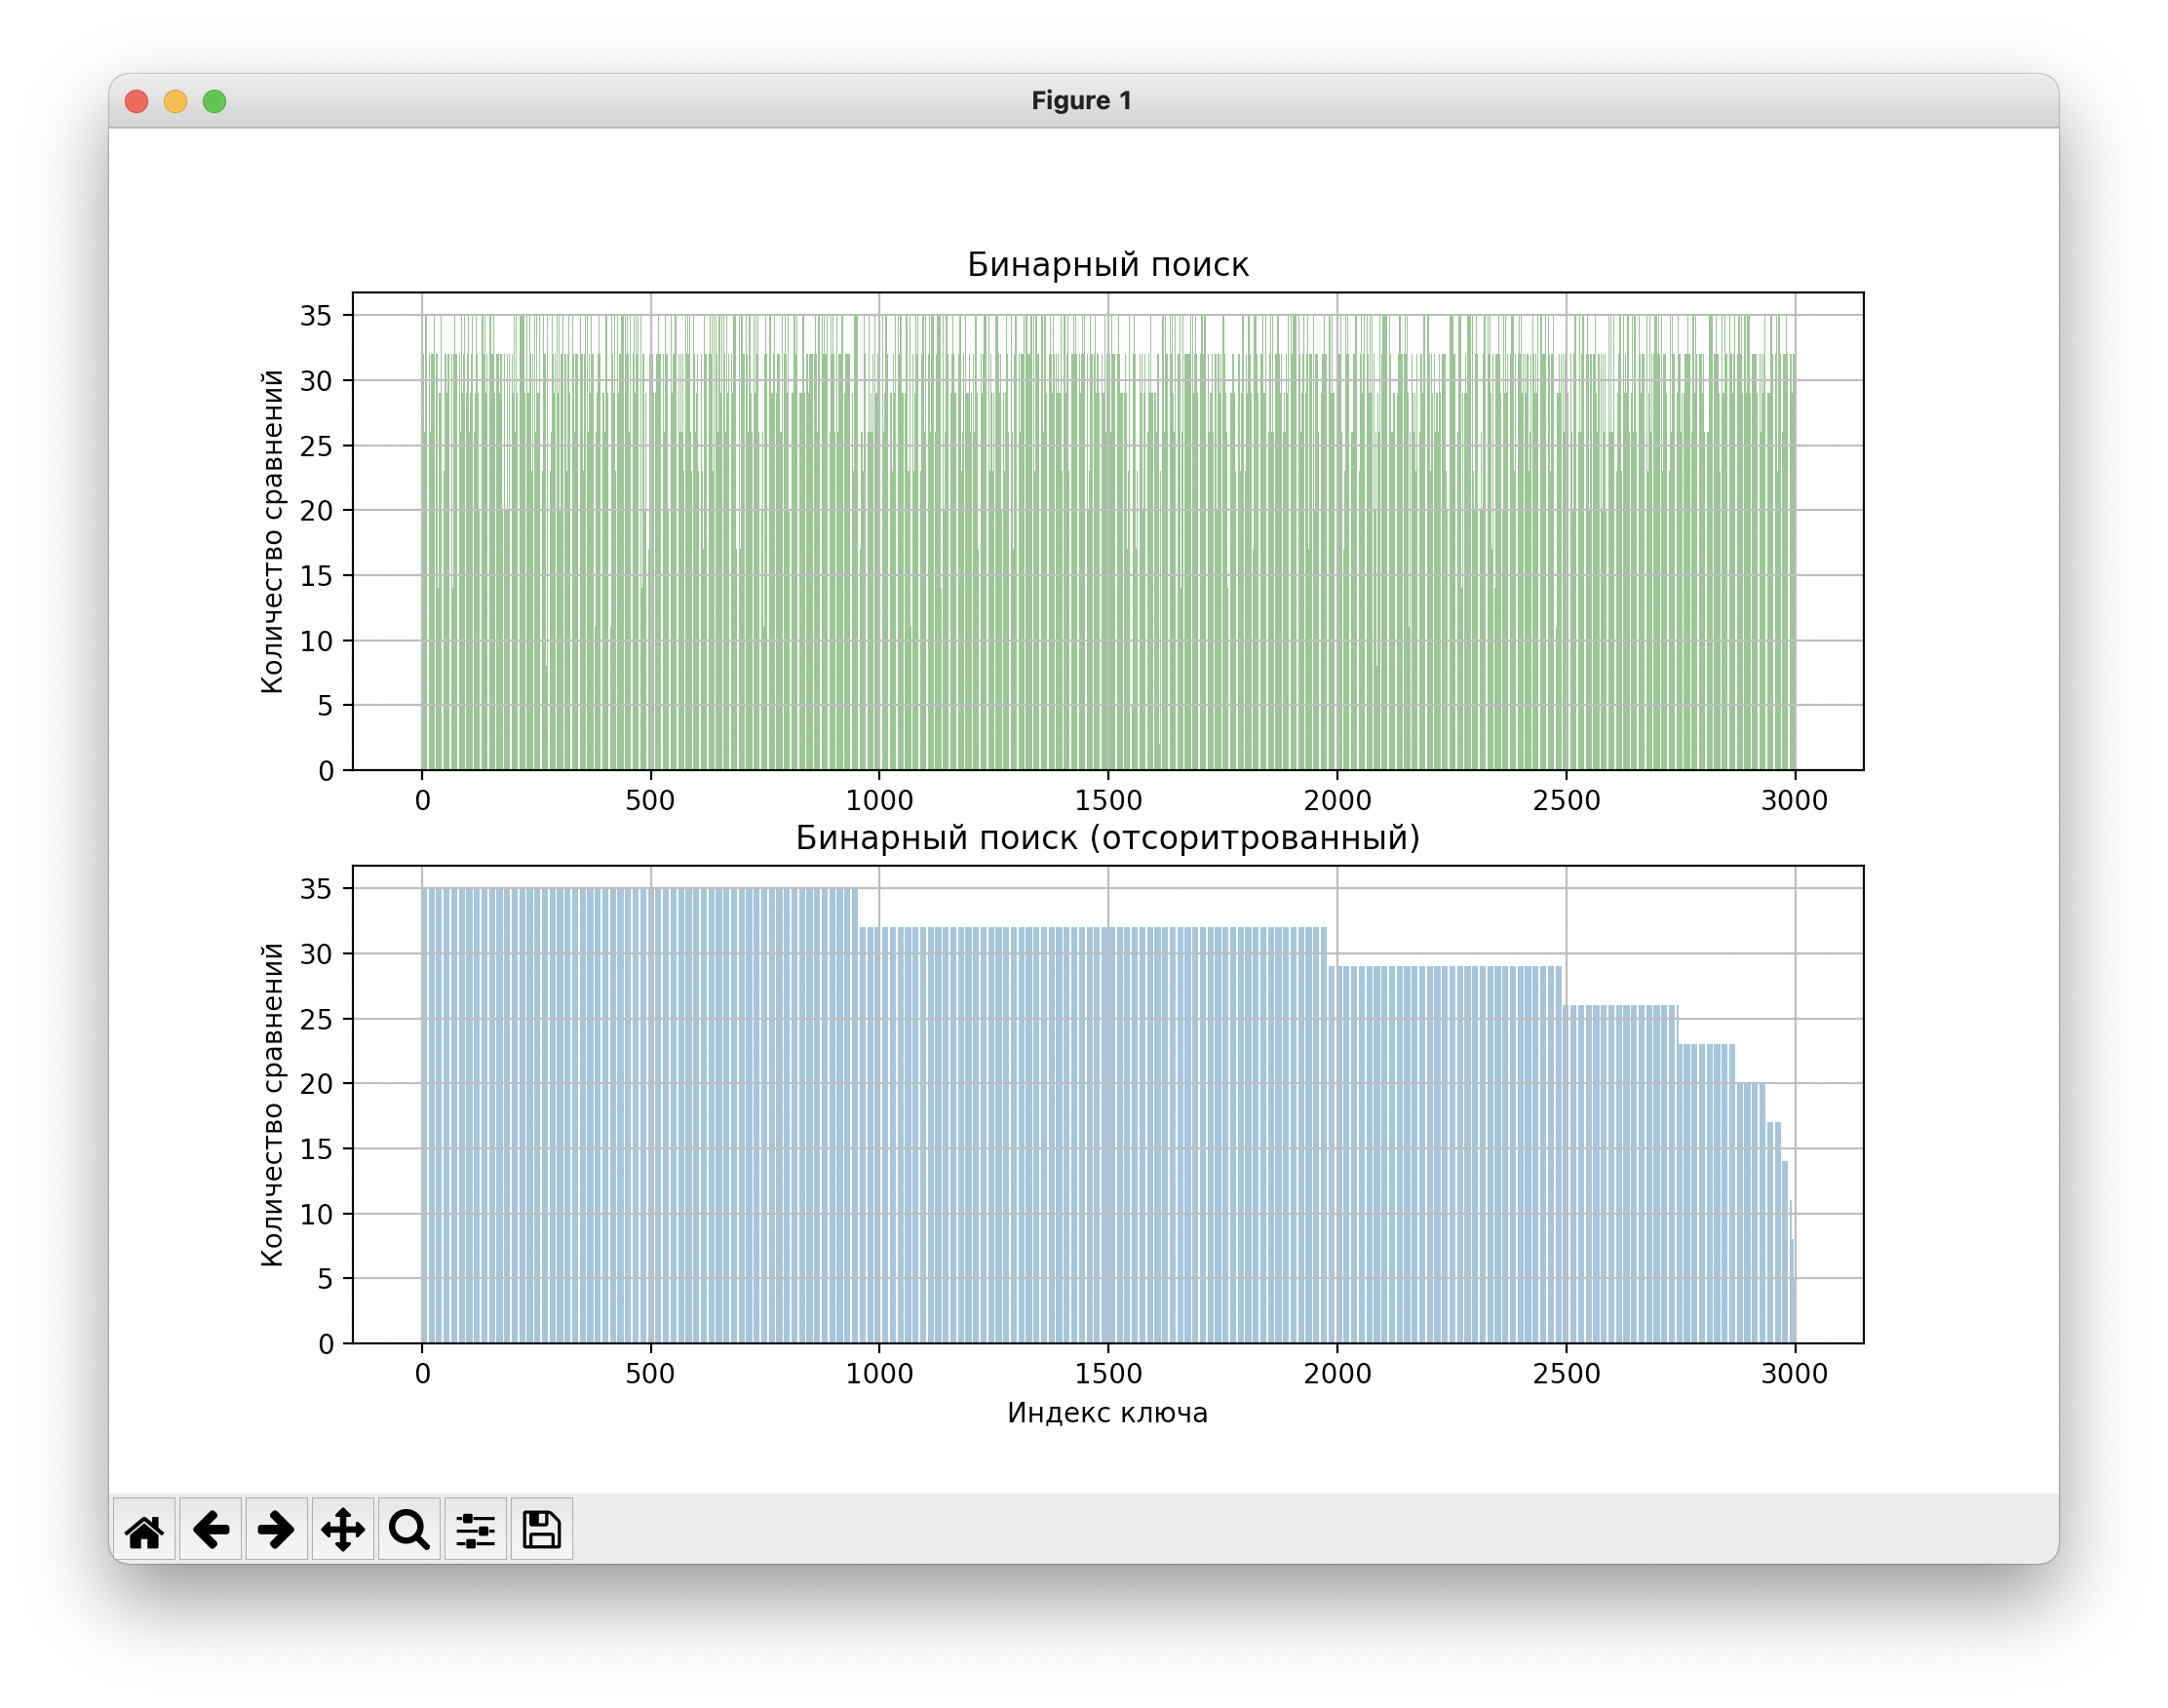
\includegraphics[scale=0.45]{img/graph_binary_search.png}
	\caption{Кол-во сравнений при поиске ключа в словаре (бинарным поиском)}
	\label{fig:graph_binary_search}
\end{figure}

\clearpage

\begin{figure}[h]
	\centering
	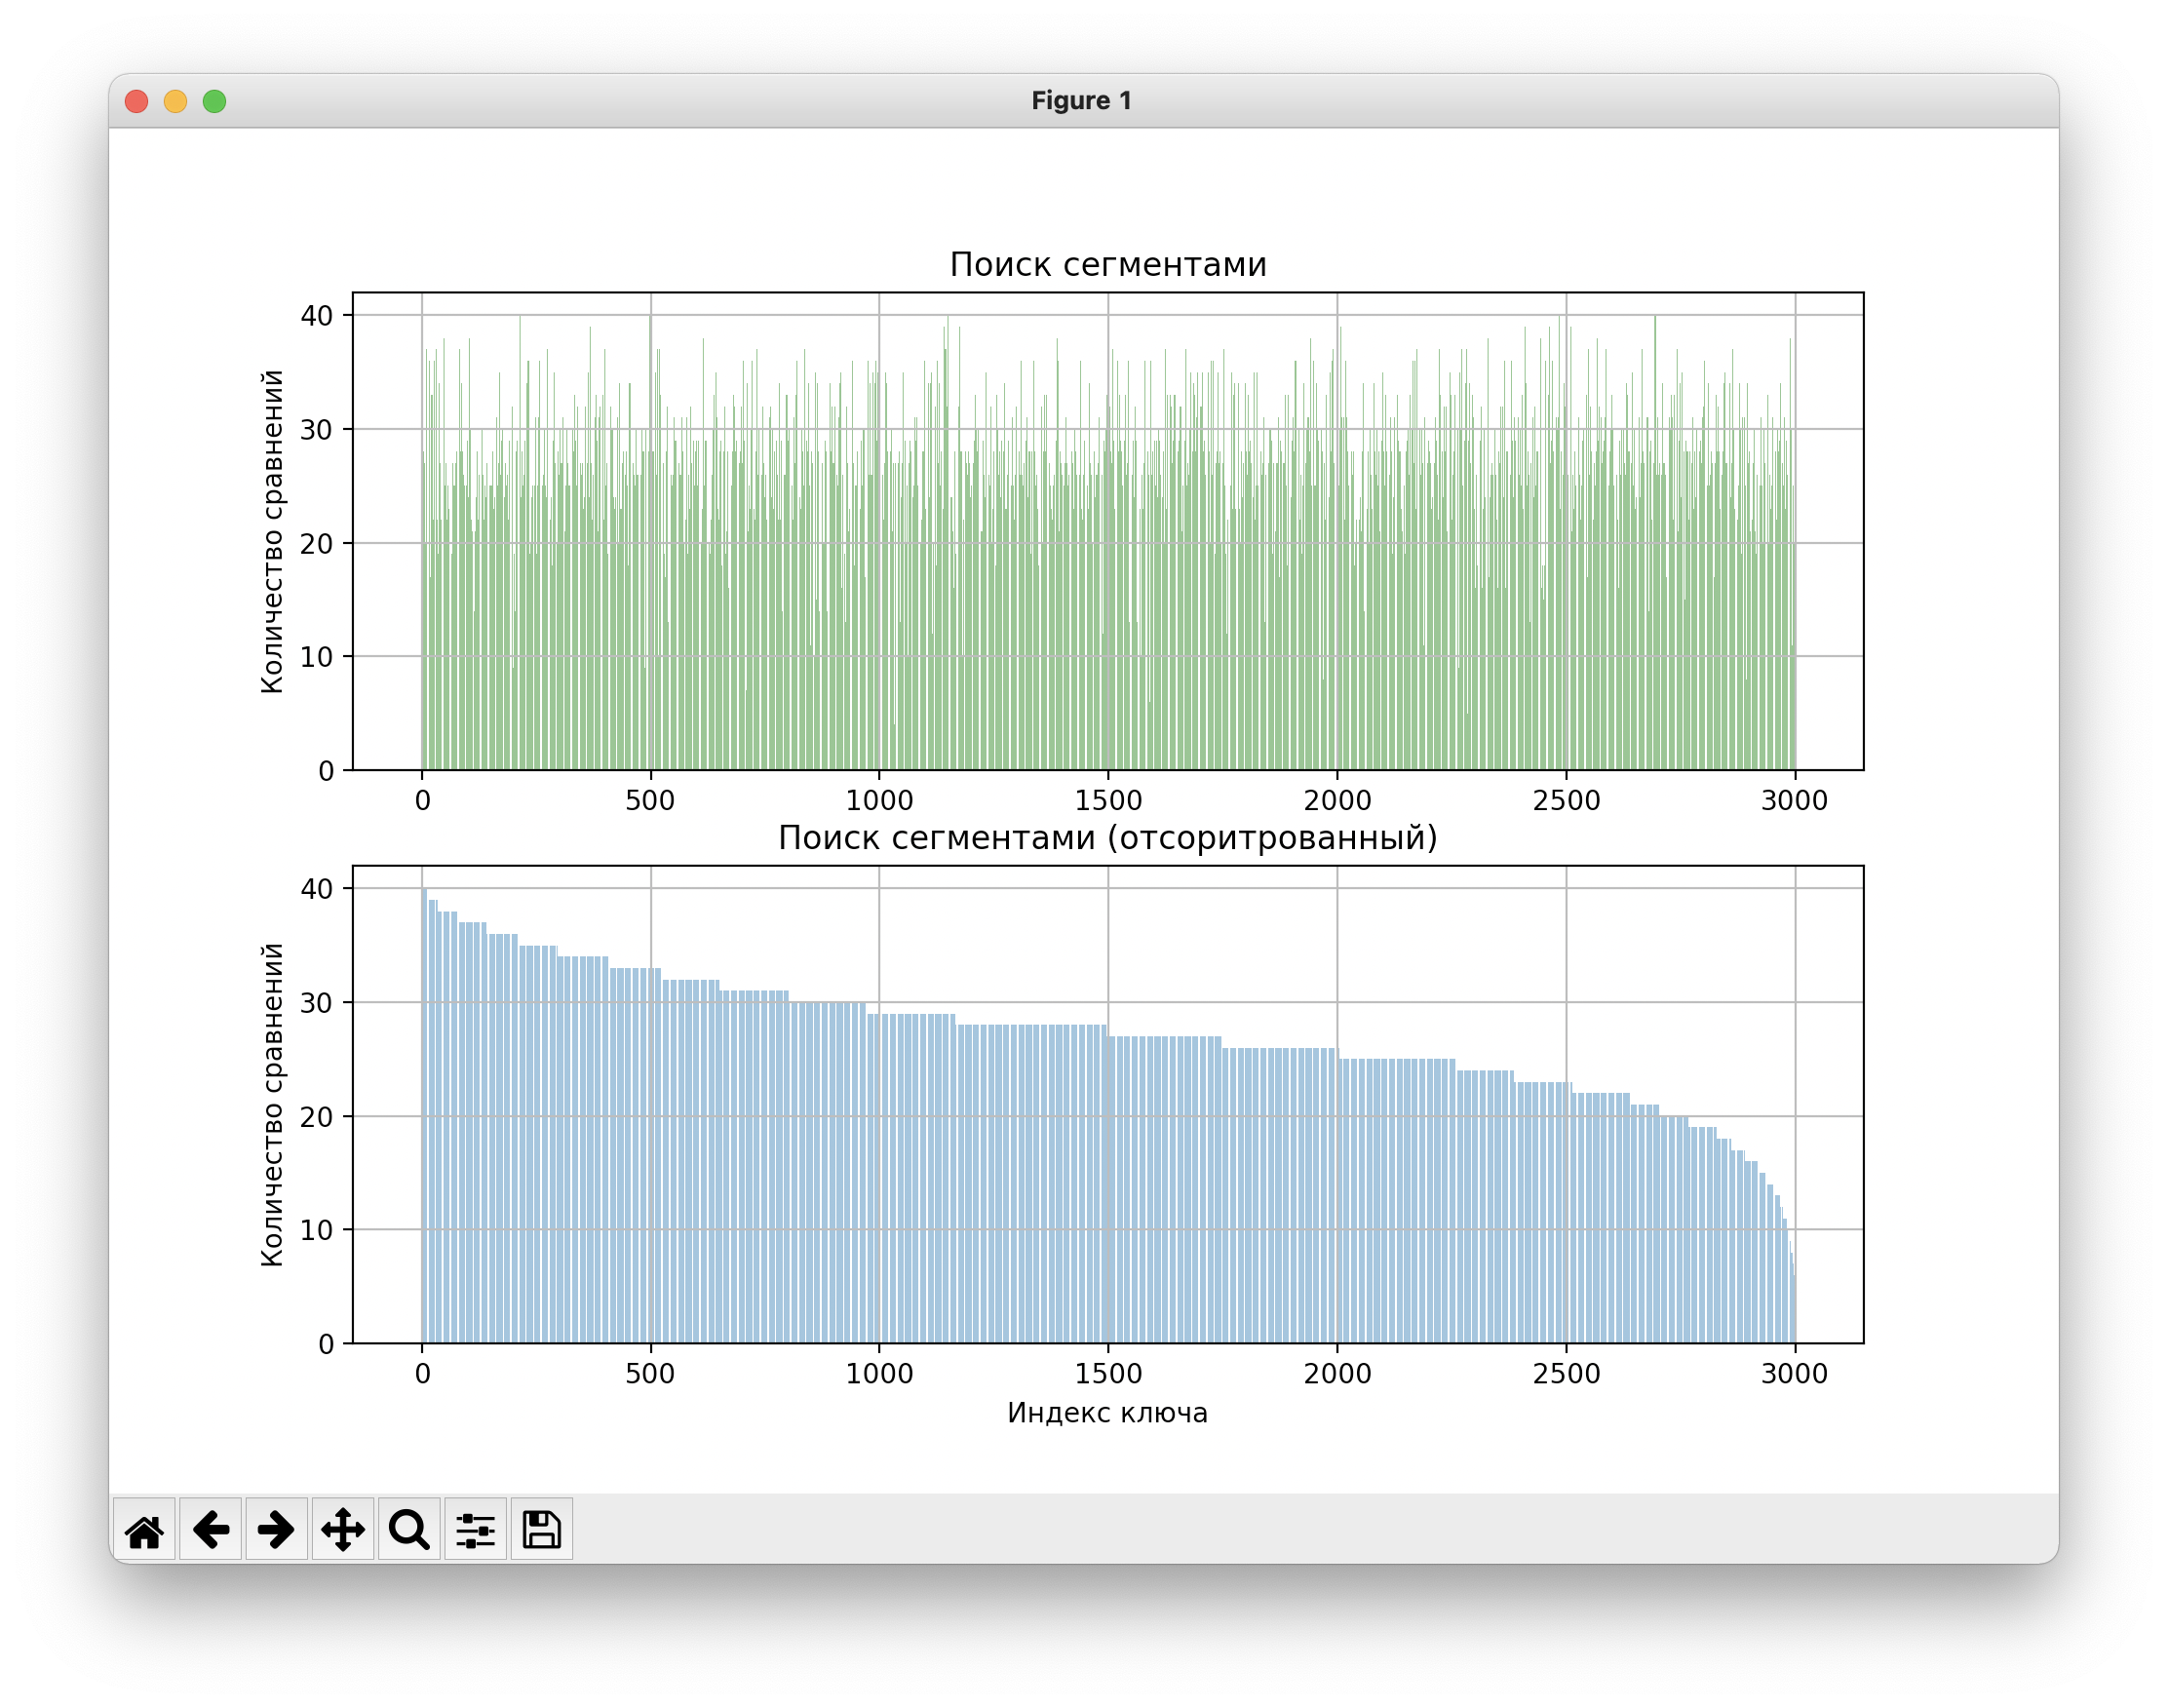
\includegraphics[scale=0.45]{img/graph_segment_search.png}
	\caption{Кол-во сравнений при поиске ключа в словаре (поиском сегментами)}
	\label{fig:graph_segment_search}
\end{figure}

\clearpage

\section{Вывод}

В этом разделе были указаны технические характеристики машины, на которой происходило сравнение времени работы алгоритмов поиска в словаре (полным перебором, бинарным поиском, поиском сегментами), а также кол-ва сравнений, используемых каждым из алгоритмов.



В результате замеров времени было установлено, что 
алгоритм поиска сегментами работает лучше остальных алгоритмов на всех ключах (В 5.1 раз быстрее алгоритма бинарного поиска при любом значении ключа и в 15.8 раз быстрее алгоритма поиска полным перебором на индексе ключа - 1000 и в 38.1 раз быстрее на индексе ключа - 3000). Стоит отметить, что алгоритм бинарного поиска и алгоритм поиска сегментами имеют примерно одинаковое время поиска каждого ключа, а скорость алгоритма полного перебора зависит от положения ключа в словаре (чем дальше ключ от начала словаря, тем дольше будет работать поиск).

Также в результате измерения кол-ва сравнений, используемых каждым из алгоритмов было установлено, что 
алгоритм поиска сегментами в среднем использует минимальное кол-во сравнений для нахождения значения ключа - 28 (алгоритм бинарного поиска использовал - 32 сравнения, а алгоритм поиска полным перебором - 1500). При этом максимальное кол-во сравнений для алгоритма поиска сегментами составило 40 сравнений, для алгоритма бинарного поиска - 35 сравнений, а для алгоритма поиска полным перебором - 3000 сравнений.





\chapter*{Заключение}
\addcontentsline{toc}{chapter}{Заключение}

Было экспериментально подтверждено различие во временной эффективности алгоритмов поиска в словаре (полным перебором, бинарным поиском, поиском сегментами). В результате исследований можно сделать вывод о том, что при возможности стоит использовать алгоритм поиска сегментами, так как он работает лучше остальных алгоритмов на всех ключах (В 5.1 раз быстрее алгоритма бинарного поиска при любом значении ключа и в 38.1 раз быстрее алгоритма поиска полным перебором на индексе ключа - 3000), а так же он в среднем использует минимальное кол-во сравнений (28). Однако стоит помнить, что для алгоритма поиска с помощью сегментов требуется разбить словарь на части (сегменты), что может быть не всегда удобно.


\vspace{5mm}

В ходе выполнения данной лабораторной работы были решены следующие задачи:
\begin{itemize}
	\item изучены алгоритмы поиска в словаре (полным перебором, бинарным поиском, поиском сегментами);
	\item применены изученные основы для реализации описанных алгоритмов;
	\item произведен сравнительный анализ алгоритмов поиска в словаре;
	\item экспериментально подтверждено различие во временнoй эффективности рассматриваемых алгоритмов при помощи разработанного программного обеспечения на материале замеров процессорного времени;
	\item произведен сравнительный анализ по количеству сравнений, необходимых алгоритмам для нахождения каждого ключа в словаре;
	\item описаны и обоснованы полученные результаты в отчете о выполненной лабораторной работе.
\end{itemize}

Поставленная цель была достигнута.





\begin{thebibliography}{5}
	\bibitem{bib1}
	Словари [Электронный ресурс]. Режим доступа: \url{https://younglinux. info/python/dictionary} (дата обращения: 10.12.2021).
	\bibitem{bib2}
	Полный перебор [Электронный ресурс]. Режим доступа: \url{http:// skud-perm.ru/posts/polnyj-perebor} (дата обращения: 10.12.2021).
	\bibitem{bib3}
	Бинарный поиск [Электронный ресурс]. Режим доступа: \url{https:// prog-cpp.ru/search-binary/} (дата обращения: 10.12.2021).
	\bibitem{bib4}
	Нильсон Н. Искусственный интеллект. Методы поиска решений. 1973.
	\bibitem{bib5}
	Welcome to Python [Электронный ресурс]. Режим доступа: \url{https://www.python.org} (дата обращения: 18.10.2021).
	\bibitem{bib6}
	time — Time access and conversions [Электронный ресурс]. Режим доступа: \url{https://docs.python.org/3/library/time.html#functions} (дата обращения: 18.10.2021).
	\bibitem{bib7}
	macOS Monterey - Apple(RU) [Электронный ресурс]. Режим доступа: \url{https://www.apple.com/ru/macos/monterey/} (дата обращения: 14.10.2021).
	\bibitem{bib8}
	Intel [Электронный ресурс]. Режим доступа: \url{https://www.intel.ru/content/www/ru/ru/products/details/processors/core/i5.html} (дата обращения: 14.10.2021).
\end{thebibliography}

\addcontentsline{toc}{chapter}{Список литература}

\end{document}
